\documentclass{article}
\usepackage{graphicx} % Required for inserting images

\title{Assignment 4 - Bragg's Law}
\author{Devanarayanan V S MM22B025}
\date{15 June 2023}

\begin{document}

\maketitle
\section{MM22B025}
\subsection{Definition}
When the X-ray is incident onto a crystal surface, its angle of incidence, $\theta$, will reflect with the same angle of scattering, $\theta$. And, when the path difference, d is equal to a whole number, n, of wavelength, $\lambda$, constructive interference will occur. The relation between the wavelength $\lambda$, order, path difference and $\theta$ is called the Bragg's equation.
\\
\subsection{Formula}
\begin{equation}
\centering
n\lambda = 2dsin\theta \footnote{Reference: https://byjus.com/physics/braggs-law/}
\end{equation}
where, \\
$\lambda$ = Wavelength of incident ray\\
$\theta$ = Angle of incidence of ray\\
d = path difference
n = order of x-rays

\subsection{Representation}
\centering
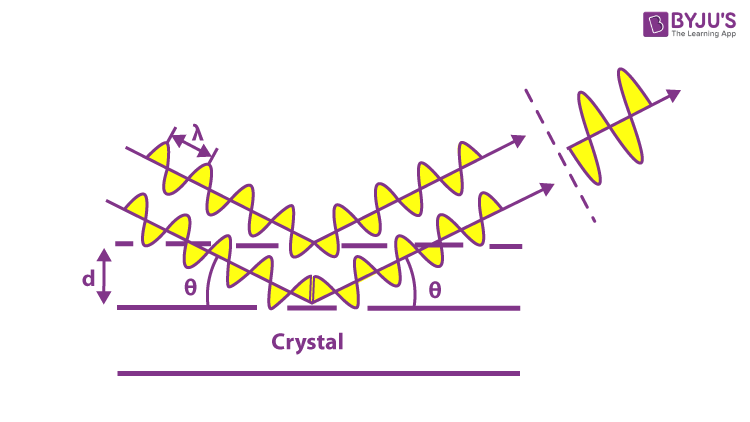
\includegraphics[width=0.65\textwidth]{braggs.png}\\
Bragg's law Representation\\
\end{document}
